\begin{minipage}[b]{.8\textwidth}
\begin{Exercise}[label = negr, origin = Aaron Wild, difficulty = 3, title = negativer Brechungsindex]
	Für Licht bestimmter Wellenlänge ist es möglich, Materialien zu konstruieren, die einen negativen Brechungsindex haben. Es gilt dann zwar immer noch das Reflexionsgesetz, allerdings ist der Ausfallswinkel, $\beta$ in der Skizze, jetzt negativ.\\
	Wir betrachten jetzt einen Swimmingpool, der mit einer Flüßigkeit mit einem Brechungsindex $n_2<0$ gefüllt ist. 
\end{Exercise}
\end{minipage}
\hfill
\begin{minipage}[b]{0.2\textwidth}
	\centering
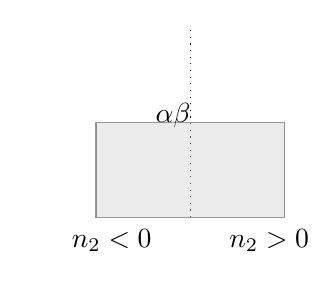
\begin{tikzpicture}
	\tkzDefPoint(-1,1){A}
	\tkzDefPoint(0,0){O}
	\tkzDefPoint(-1,-1){a}
	\tkzDefPoint(0,1){B}
	\tkzDefPoint(0,-1){b}
	
	\tkzDefPoint(1,-1){c}
	
	
	\tkzMarkAngle[scale = .75](B,O,A)
	\tkzLabelAngle(B,O,A){$\alpha$}
	\tkzMarkAngle[scale = .75](a,O,b)
	\tkzLabelAngle(a,O,b){$\beta$}
	
	\tkzDrawSegment[->](A,O)
	\tkzDrawSegment[->](O,a)
	
	\tkzDrawSegment[dashed,->](O,c)
	\draw[dotted](0,-1.2) -- (0,1.2);
	
	\filldraw[draw = black, fill = black!20, opacity = 0.4] (-1.2,0) rectangle (1.2,-1.2);
	
	\node at (-1,-1.5){$n_2<0$};
	\node at (1,-1.5){$n_2>0$};
\end{tikzpicture}
\end{minipage}